\chapter{Solution}
\label{cha:solution}

This chapter describes the methods used to build the final predictive model. As stated previously, the main goal of this research is to optimize the number of open checkouts while maintaining the waiting times under a predetermined threshold. In order to reach it, the final model is composed of different submodules that cooperates sequentially, so that the results of a submodule are used as input to the next one, as shown in Figure \ref{fig:model_architecture}. First, the \emph{measured inflow rate} of the recent past is combined with a \emph{forecasted inflow rate} of the immediate future. These values, combined with a \emph{dwell time forecast}, are used to obtain a prediction of the \emph{arrival rate at the checkouts}. The arrival rate, the number of \emph{open counters} and the approximated \emph{service rate} are then processed with queueing theory techniques to calculate the expected queue length for a given interval. Finally, different values for the number of available checkouts can be tested to obtain the minimum staff allocation that ensures that the predefined maximum queue length limit is not exceeded.

\begin{figure}[H]
  \begin{center}
    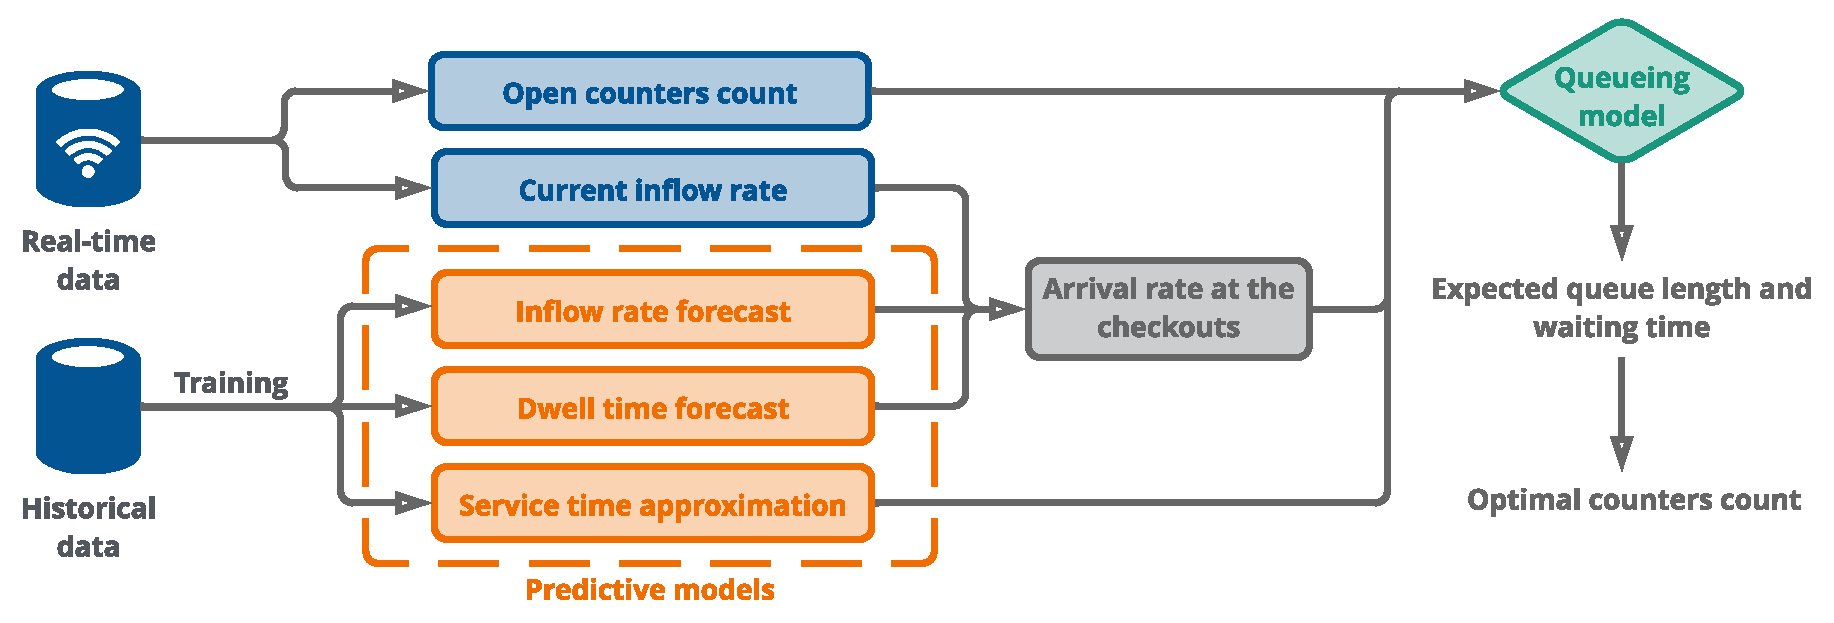
\includegraphics[width=1\textwidth]{img/model_architecture.pdf}
  \end{center}
  \caption{The final architecture of the predictive model.}
  \label{fig:model_architecture}
\end{figure}

\section{Inflow rate forecast}
\label{sec:inflow_rate_forecast}

Since the inflow rate can be expressed as a time series, different time series predictive models, already presented in Section~\ref{sec:time_series_forecasting}, were tested. This section discusses the implementation details of these models, while a comparison of the obtained results and performances is presented in Section~\ref{sec:inflow_rate_forecast_results}

\subsection{Persistence model}
\label{subsec:persistence_model}

The first model presented was used only to define a performance baseline. This gave an idea of how well the other models could perform on the data and set a minimum accuracy level: if a model’s performances were worse than this baseline, it was discarded and not considered. This baseline was obtained by using a \emph{persistence model}, where the last measured value \( y_{t-1} \) is simply used as forecast for the next time interval \( t \):
\begin{equation}
  \hat{y}_t = y_{t-1}
\end{equation}

\subsection{Drift model}
\label{subsec:drift_model}

As seen in Chapter~\ref{cha:data_analysis}, the inflow rate time series presents a strong seasonal component, so basing the forecast on this repeating pattern could results in a good accuracy. The forecast values were calculated as the average of the values in the previous weeks from the same week day and time, as:
\begin{equation}
  \hat{y}_t = \hat{f}(t) = \frac{1}{N} \sum_{i=1}^{N} y_{t-iW}
\end{equation}
where \( W \) is the number of intervals in a week and \( N \) is the number of previous weeks considered. Since we used 10-minute intervals, \( W = 1008 \). This method is accurate only if the cyclic patterns maintain the same levels every day, without any random variation.

To take in account these variations in the inflow rate, that can be caused by external factors like holidays or special promotions, a \emph{local drift} was calculated using the errors of the forecasted values for the immediate past:
\begin{equation}
  \hat{y}_t = \hat{f}(t) + \frac{1}{M} \sum_{i=1}^{M} y_{t-i} - \hat{f}(t-i)
\end{equation}
were \( M \) is the number of previous steps to be considered by the drift. We can denote this model as \( \text{Drift}(N, M) \). By doing this, the forecasts are progressively adjusted to the current traffic level while still taking in consideration the seasonal cyclic behavior.

\subsection{Autoregressive Neural Network model}
\label{subsec:artificial_neural_network_model}

As stated in Section~\ref{subsec:artificial_neural_networks}, artificial neural networks are a popular and effective technique for time series forecasting. In the same section, \emph{autoregressive neural networks} were introduced with the notation \( \text{AR-NN}(p, P, k)_m \).

Since the inflow rate's values present a strong correlation with the previous values, as seen in Section~\ref{subsec:inflow_rate_autocorrelation}, the time series is non-stationary, and therefore the dataset must be rendered stationary before training the model. This was done by \emph{differencing} the time series, i.e. by calculating the difference between consecutive observations (also called \emph{first-order differencing}). Each value of the differenced time series can be written as \( y'_t = y_t - y_{t-1} \). This transformation can help stabilize the mean of the time series, reducing the effects of trend and seasonalities. Since the time series present a strong seasonal component, a seasonal differencing was also applied, written as \( y'_t = y_t - y_{t-m} \), where \( m \) is the number of lags in a seasonal cycle. A daily seasonal cycle was taken in account, so \( m = 144 \). Both differentiations were applied to obtain stationarity, thus each observation of the final time series used to train the model was calculated as:
\begin{equation}
  y''_t = y'_t - y'_{t-1} = (y_t - y_{t-m}) - (y_{t-1} - y_{t-m-1})
\end{equation}
The ACF analysis of the differenced time series in Figure~\ref{fig:stationary_inflow_rate_acf} shows that this approach is effective in making the time series stationary.

\begin{figure}
  \begin{center}
    \inputpgf{img}{stationary_inflow_rate_acf.pgf}
  \end{center}
  \caption{The ACF of the stationarized inflow rate time series. In comparison to the non-stationary ACF (see Figure~\ref{fig:inflow_rate_acf}), there is no visible seasonality.}
  \label{fig:stationary_inflow_rate_acf}
\end{figure}

As stated in Section~\ref{subsec:artificial_neural_networks}, given a target value \( y_{t+1} \), each sample in input can be written as:
\[
  (y_{t}, y_{t-1}, ..., y_{t-p}, y_{t-m}, y_{t-2m}, ..., y_{t-Pm})
\]

The model used an MSE (Mean Squared Error) loss function and a \emph{sigmoid} activation function. The ANN was trained over a batch size of \( 24 \cdot 6 = 144 \) samples, that is the number of observations in a day. The training was then repeated for a total of \( 100 \) epochs. Various parameters values for \( p \), \( P \) and \( k \) were tested and the model with the best performance was used. The obtained results and accuracy are discussed in Section~\ref{sec:inflow_rate_forecast_results}.

\subsection{SARIMA model}
\label{subsec:sarima_model}
In Section~\ref{subsec:arima_models} the ARIMA model and some of its evolutions were introduced. Since the inflow rate presents a strong daily seasonal pattern, as seen in Section~\ref{subsec:inflow_rate_autocorrelation}, the SARIMA model was chosen as a possible forecasting method. This model has different parameters that must be configured correctly in order to achieve a good prediction accuracy:
\begin{itemize}
  \item \( p \): autoregressive order;
  \item \( d \): degree of differencing;
  \item \( q \): moving average order;
  \item \( P \): seasonal autoregressive order;
  \item \( D \): seasonal degree of differencing;
  \item \( Q \): seasonal moving average order;
  \item \( m \): number of time steps in the seasonal period.
\end{itemize}

The parameters configuration can be written as \( \text{SARIMA}(p,d,q)(P,D,Q)_m \). For some of these parameters, the optimal values can be determined by the analysis of the time series, while the only possible approach for the others is to try different values and select the ones that minimize the forecasting errors. By the results obtained in Chapter~\ref{cha:data_analysis}, we can set:
\begin{itemize}
  \item \( d = 1 \) and \( D = 1 \) for respectively first-order and seasonal differencing. By doing this, we achieve the same type of differencing explained in the previous section;
  \item \( q = 6 \) and \( Q = 3 \), obtained by the PACF analysis of the differenced time series. Specifically, the plot shows an exponential decay on the seasonal lags of the PACF (e.g at lags 144, 288, ...). For this reason, the number of significant autocorrelation coefficients gives a good approximation for \( q \) and \( Q \)~\cite{hyndman2018};
  \item \( m = 144 \), that is the daily seasonal cycle length, i.e. the number of 10-minute intervals in a day.
\end{itemize}

In 2007, Hyndman et al.~\cite{hyndman2007} proposed the \emph{Hyndman-Khandakar algorithm}, which combines unit root tests, minimization of the \emph{Akaike’s Information Criterion} (AIC) and \emph{Maximum Likelihood Estimation} (MLE) to automatically determine the best parameters for the SARIMA model. While this method is very computational expensive and does not always returns the best configuration, it removes a lot of the steps and trials involved in the parameters determination, simplifying the whole process. By using this technique, the parameters values presented previously were confirmed to be the optimal ones. Moreover, the results showed that by using \( p = 0 \) and \( P = 0 \) the best accuracy was obtained.

\section{Arrival rate forecast}
\label{sec:arrival_rate_forecast}

Once a predictive model was defined, the measured and forecasted inflow rates were combined and used to get a prediction of the \emph{arrival rate} at the checkouts. Since the inflow rate into the shop appears with a delay at the checkout area, and this delay is the customer's dwell time, a time-dependent probability density function \( p_t(\tau) \) is required, where \( \tau \) is the expected dwell time of a customer~\cite{aksu}.

In Section~\ref{sec:dwell_time_inflow_rate_service_time_distributions} the general distribution of the dwell time was presented and, with the analysis of Section~\ref{sec:time_series_analysis}, it is clear that it is strongly time-dependent, thus it can be seen as a stochastic process \( \{ X_t \} \) with \( X_t \sim \text{Erlang}(k_t, n_t) \), where \( k_t = \text{E}[X_t]^2 / \text{Var}[X_t] \) and \( n_t =  \text{E}[X_t] / \text{Var}[X_t] \). Given the weekly and daily seasonality of the time series, different \( X_t \) distributions were defined for each interval on every week day, for a total of \( 7 \cdot 24 \cdot 6 = 1008 \) distributions, since 10-minute intervals were used. Each aforementioned distribution was obtained by calculating the values for \( \text{E}[X_t] \) and \( \text{Var}[X_t] \) from the observations of the previous weeks on the same interval and week day.

Let \( \lambda(t) \) be the \emph{predicted arrival rate} for the time interval \( t \), \( \Delta t \) the intervals size, \( p_t(\tau_i) \) the probability of having a dwell time of \( \tau_i \), with \( (i-1) \Delta t < \tau_i \leq i \Delta t \), and \( y_{t-i} \) the \emph{measured inflow rate} at time \( t-i \). We can approximate \( \lambda(t) \) by:
\begin{equation}
  \lambda(t) = \sum_{i=1}^{\infty} y_{t-i} \cdot p_t(\tau_i)
\end{equation}

Since after a certain \( \tau_i \) value, \( p_t(\tau_i) \) becomes irrelevant, we can limit the number of values to be considered by defining a maximum dwell time \( \tau_{max} \), that can be set either by a customizable parameter or by analyzing the dwell times distribution (e.g. by using the \emph{95th percentile}). In any case, \( \tau_{max} \) should be such that \( p_t(\tau_{max} + \Delta t) \) tends to zero. We can then rewrite the previous formula as:
\begin{equation}
  \lambda(t) = \sum_{i=1}^{K} y_{t-i} \cdot p_t(\tau_i)
  \label{eq:arrival_rate1}
\end{equation}
where \( K \) is such that \( \tau_K \leq \tau_{max} \leq \tau_{k+1} \). This equation is however applicable only if the measured values for \( y_{t-1}, y_{t-2}, ..., y_{y-K} \) are known, thus only when \( t \leq t_{now} \), where \( t_{now} \) is the current interval when those calculations are executed. If \( t > t_{now} \), a forecast of the inflow rate, as described in Section~\ref{sec:inflow_rate_forecast}, must be used to provide the missing information. For this reason, we define a function \( \text{in}(t) \) as:
\begin{equation}
  \text{in}(t) = \\
  \begin{cases}
    y_{t}       & \quad \text{if } t < t_{now} \\
    \hat{y}_{t} & \quad \text{otherwise}
  \end{cases}
\end{equation}
where \( y_t \) and \( \hat{y}_t \) are respectively the measured and predicted inflow rate at time \( t \). It shall be noted that the real measurements for an interval are available only once the said interval is ended, hence the reason for using \( y_t \) only when \( t < t_{now} \). The Equation~(\ref{eq:arrival_rate1}) is therefore rewritten as:
\begin{equation}
  \lambda(t) = \sum_{i=1}^{K} \text{in}(t-i) \cdot p_t(\tau_i)
\end{equation}

To obtain a \emph{multi-step forecast} of the next \( N \) intervals, we can directly solve a linear system of equations:
\begin{equation}
  \begin{bmatrix}
    \lambda(t)   \\
    \lambda(t+1) \\
    \vdots       \\
    \lambda(t+N)
  \end{bmatrix} =  \\
  \begin{bmatrix}
    \text{in}(t-1)     & \text{in}(t-2)     & \cdots & \text{in}(t-K)     \\
    \text{in}(t)       & \text{in}(t-1)     & \cdots & \text{in}(t-(K-1)) \\
    \vdots             & \vdots             & \ddots & \vdots             \\
    \text{in}(t+(N-1)) & \text{in}(t+(N-2)) & \cdots & \text{in}(t+(N-K))
  \end{bmatrix}
  \begin{bmatrix}
    p_t(\tau_1) \\
    p_t(\tau_2) \\
    \vdots      \\
    p_t(\tau_K)
  \end{bmatrix}
\end{equation}

Section~\ref{sec:arrival_rate_forecast_results} describes the results obtained and the accuracy of this predictive model.

\section{Queue length forecast}
\label{sec:queue_length_forecast}

This section describes the model implemented for forecasting the queue length at the checkouts. As described in Section~\ref{sec:queueing_theory}, the required variables are:
\begin{itemize}
  \item \( \lambda(t) \): arrival rate at the checkouts;
  \item \( \mu(t) \): service rate of a single checkout;
  \item \( c(t) \): total count of available checkouts (servers), also referred to as the \emph{configuration} of the checkouts.
\end{itemize}

A forecast of the arrival rate \( \lambda(t) \) has been proposed in the previous section and an approximation of the service rate \( \mu(t) \) is presented in the next section. The total number of open checkouts \( c(t) \) is the tunable parameter that can be used to evaluate the performance of different checkouts configurations.

\subsection{Service rate approximation}
\label{subsec:service_rate_approximation}

In Section~\ref{subsec:service_time_approximations}, various possible approximations for the service time were introduced. In Section~\ref{subsec:service_rate_and_open_terminals_count_approximation}, it was shown that a constant, and therefore time-independent, service rate could be used without losing precision. This constant service rate was obtained by investigating the time spent in idle by each terminal, which was determined by the analysis of the inter-exit times.

As described in Section~\ref{subsec:service_time_approximations}, when the time spent in idle by the counters’ staff becomes insignificant, i.e. when it approaches a value of zero, the customers’ inter-exit times can give a good approximation of the actual time spent serving each customer in the queue. Since the idle time is not an available measurement, this was achieved by using the hours with peaks in the arrival rate at the checkouts as an indicator of low idle times. A threshold value \( \lambda_{max} \) was defined, such that when it is exceeded by the actual arrival rate, i.e. when \( \lambda_t \ge \lambda_{max} \), the time \( t \) can be considered as a period with high traffic density, and therefore included in the aforementioned approximation. An average of the measured inter-exit times during these high traffic periods was then calculated and used as \emph{service time} \( S \) of a single counter. The \emph{service rate} \( \mu \) was then obtained from \( S \) using Eq.~(\ref{eq:service_rate}). In Section~\ref{sec:queue_length_forecast_results} the results of this approximation are presented.

\subsection{Queue length approximation}
\label{subsec:queue_length_approximation}

As described in Section~\ref{sec:queueing_theory}, the standard queueing theory does not support time-varying arrival rates with temporal overloading. The only approach that seemed to fit the context of this research was the \emph{Stationary Backlog-Carryover} (SBC) approach, proposed by Stolletz in 2008~\cite{stolletz}. SBC is based on a \( M/M/c/c \) model, in which a maximum number of \( c \) customers can be in the queue at any time and any further arrival is considered \emph{blocked} (i.e. lost), and uses an artificial arrival rate \( \widetilde{\lambda}_t \) to take in account the temporal overloading of the queue, allowing standard queueing models to be used. \( \widetilde{\lambda}_t \) consists of both the average arrival rate \( \lambda_t \) and the \emph{backlog rate} of the previous period \( b_{t-1} \), that is the rate of customers leaving the system due to blocking in the former period.

Let \( P_t(B) \) be the steady-state probability of blocking for the \( M/M/c/c \) model in period \( t \) with artificial arrival rate \( \widetilde{\lambda}_t \). The backlog rate \( b_t \) is given by:
\begin{equation}
  b_t = \widetilde{\lambda}_t \cdot P_t(B)
\end{equation}

These blocked customers are carried over into the period \( t+1 \), which results in the artificial arrival rate \( \widetilde{\lambda}_{t+1} \). Starting with \( \widetilde{\lambda}_1 = \lambda_1 \) and \( b_0 = 0 \), we can define the artificial arrival rate recursively through:
\begin{equation}
  \widetilde{\lambda}_t = \lambda_t + b_{t-1} = \lambda_t + \widetilde{\lambda}_{t-1} \cdot P_{t-1}(B)
\end{equation}

By doing this, the customers not served in period \( t-1 \) are evenly spread over period \( t \). The probability \( P_t(B) \) is obtained by the \emph{Erlang’s loss} formula:
\begin{equation}
  P_t(B) = \frac{(\widetilde{\lambda}_t / \mu_t)^{c_t}}{c_t!\sum_{k=0}^{c_t} \frac{(\widetilde{\lambda}_t / \mu_t)}{k!}}
\end{equation}

The expected servers utilization \( \rho_t \) can be then calculated as:
\begin{equation}
  \rho_t = \frac{\widetilde{\lambda}_t(1 - P_t(B))}{c_t\mu_t} = \frac{\widetilde{\lambda}_t - b_t}{c_t\mu_t} = \frac{\lambda_t + b_{t-1} - b_t}{c_t\mu_t}
  \label{eq:servers_utilization}
\end{equation}

Stolletz proposed two different approximations for the expected number of customers in the queue, the first based on a \emph{Modified Arrival Rate} (MAR) and the second based on \( \rho_t \) and \( b_t \)~\cite{stolletz}.

The MAR approach uses an \( M/M/c/\infty \) queueing model, with the same utilization factor \( \rho_t \) of the \( M/M/c/c \) model analyzed in the previous step. To do so, a modified arrival rate \( \lambda_t^{MAR} \) is chosen such that the model reach the approximated \( \rho_t \) obtained by Eq.~(\ref{eq:servers_utilization}), in particular:
\begin{equation}
  \lambda_t^{MAR} = \rho_t c_t \mu_t
\end{equation}

Applying Eq.~(\ref{eq:servers_utilization}) results in:
\begin{equation}
  \lambda_t^{MAR} = \lambda_t + b_{t-1} - b_t
\end{equation}

The expected number of customers in the system \( Ls_t \) can be then obtained by solving the specific formula for the \( M/M/c/\infty \) model~\cite{kleinrock}:
\begin{equation}
  Ls_t^{MAR} = c_t\rho_t + \frac{\rho_t}{1-\rho_t} \pi_{c_t^+}
\end{equation}
where \( \pi_{c_t^+} \) is the probability of having all the \( c_t \) servers occupied:
\begin{equation}
  \pi_{c_t^+} = \frac{(c_t\rho_t)^{c_t}}{c_t!(1-\rho_t)}\pi_0
\end{equation}
and \( \pi_0 \) denotes the probability of having \( 0 \) customers in the system:
\begin{equation}
  \pi_0 = \left[ \sum_{k=0}^{c_t-1} \frac{(c_t\rho)^k}{k!} + \frac{(c_t\rho)^{c_t}}{c_t!} \frac{1}{1-\rho_t} \right]^{-1}
\end{equation}

The second proposed approach approximates the expected queue length with the number of backlogged customers (\emph{A1 approximation}). The backlog rate \( b_t \) is multiplied by the period length \( \Delta t \) to obtain the number of waiting customers at the end of period \( t \). The expected queue length \( Lq_t^{A1} \) is then given by:
\begin{equation}
  Lq_t^{A1} = b_t \Delta t
\end{equation}
and the total number of customers in the system \( Ls_t^{A1} \) by:
\begin{equation}
  Ls_t^{A1} = Lq_t^{A1} + c_t \rho_t
\end{equation}

However, they showed that the expected queue length is often overestimated by the A1 approximation. An improvement was obtained by reducing the approximated \( Lq_t^{A1} \) value by the expected number of non-busy servers \( c_t (1 - \rho_t) \) (\emph{A2 approximation}), such that:
\begin{equation}
  Lq_t^{A2} = max\{0, Lq_t^{A1} - c_t (1 - \rho_t)\}  \;\;\;\text{and}\;\;\;  Ls_t^{A2} = Lq_t^{A2} + c_t \rho_t
\end{equation}

Once the number of customers in queue has been determined, Little’s Law~(\ref{eq:little_law})~\cite{little} can be used to calculate the expected queue and system waiting times, respectively \( Wq_t \) and \( Ws_t \), as:
\begin{equation}
  Wq_t = Lq_t / \lambda^{MAR}_t  \;\;\;\text{and}\;\;\;  Ws_t = Ls_t / \lambda^{MAR}_t
\end{equation}

The results and performances of each approximation are discussed in Section~\ref{sec:queue_length_forecast_results}.

\section{Checkouts optimization}
\label{sec:checkouts_optimization}

In the previous section, various approximations for the average queue length were discussed. In this section, these approximations are used to compute the optimal number of checkouts that should be opened to maintain an acceptable service level while reducing the manned staff’s idle time.

\subsection{Optimal checkouts configuration}
\label{subsec:optimal_checkouts_configuration}

The optimal number of open checkouts \( c \) for the next future period \( t+1 \) should be as low as possible, but still enough to maintain the queue length under a predetermined acceptable threshold \( Ls_{max} \). The problem can be alternatively expressed as “find the minimum value for \( c \) such that \( Ls(c) \leq Ls_{max} \) and \( 1 \leq c \leq c_{max} \)”, where \( Ls(c) \) is the expected queue length having \( c \) servers, calculated using one of the methods presented in the previous section, and \( c_{max} \) is the total number of available checkouts in the supermarket. Given the complexity of the model, different values for \( c \) are tried with the queue length forecast equations until the best value is found, starting with \( c = c_{now} \), where \( c_{now} \) is the current number of open counters. Algorithm~\ref{alg:checkouts_optimization} shows a possible implementation of this process.
\begin{algorithm}
  \SetAlgorithmName{Algorithm}{} \;
  $ c \gets c_{now}$\;
  \If{\FuncSty{Ls($c$)} $ > Ls_{max}$}{
    \While{$ c \leq c_{max} $ \KwSty{and} \FuncSty{Ls($c$)} $ > Ls_{max} $}{
      $ c \gets c + 1 $\;
    }
  }
  \Else{
    \While{$ c \ge 1 $ \KwSty{and} \FuncSty{Ls($c$)} $ < Ls_{max}$}{
      $ c \gets c - 1 $\;
    }
    $ c \gets c + 1 $\;
  }
  \caption{\label{alg:checkouts_optimization}Determine the optimal checkouts configuration.}
\end{algorithm}

Alternatively, a maximum waiting time \( Ws_{max} \) can be used as threshold, instead of \( Ls_{max} \). In that case the algorithm remains the same but with \( Ls(c) \) and \( Ls_{max} \) respectively replaced by \( Ws(c) \) and \( Ws_{max} \).

\subsection{Opening/closing fluctuations control}
\label{subsec:opening_closing_fluctuations_control}

In order to avoid opening and closing checkouts too frequently, an additional control has to be implemented. For example, it should be possible to exceed the maximum waiting time limit for a short period of time, to avoid opening a new counter that would not be fully used after this short high-traffic period is ended. The system should therefore evaluate if it is necessary to change the checkouts configuration in a new state which is persistent for a relevant amount of time, or if the increased traffic is transient and would last for just a short period. If such trend is not persistent, there should be no changes in the actual number of open checkouts.

To do so, a multi-step forecast must be implemented. For example, let \( \hat{c}_{t+1} \) be the forecasted optimal configuration for the next interval and \( c_t \) the current configuration: if \( \hat{c}_{t+1} > c_t \), the values for \( \hat{c}_{t+2}, \hat{c}_{t+3}, ..., \hat{c}_{t+n} \) must also be computed to make a decision. If the trend is not persistent, e.g. \( \hat{c}_{t+2} = c_t \), there should be no changes in the configuration. We can thus define two store-based customizable parameter:
\begin{itemize}
  \item \( n \): the number of future steps that shall be analyzed, with \( n \ge 2 \);
  \item \( m \): the minimum number of steps that should present the new trend level, with \( m \le n \).
\end{itemize}

If at least \( m \) of the \( n \) predicted values present a persistent trend, the checkouts configuration shall be adjusted accordingly. Otherwise, the trend variation can be considered temporary and therefore ignored.

\clearpage